\chapter{Formalismen}
\label{ch:formalism}
In dit hoofdstuk wordt er gekeken naar formalisme binnen interactive story telling. Er wordt een voorstel gedaan voor de softwarearchitectuur van de nieuwe editor om meerdere formalisme te ondersteunen in één omgeving. Deze softwarearchitectuur betreft het leggen van een scheiding tussen de editor en het achterliggende formalisme. Het ondersteunen van meerdere formalismen maakt het onderhouden van twee aparte editors overbodig.

\section{Formalismen binnen interactive story telling}
\subsection{De rol van formalisme}
Het formaliseren van het narratief speelt een grote rol tijdens het ontwikkelproces van narrative games. Volgens een vastgesteld formalisme wordt er betekenis gegeven aan de structuur achter het narratief. Een formalisme is een theorie die bepaalde richtlijnen afdwingt en waarde koppelt aan syntax. In \autoref{fig:simplestorytree} is een voorbeeld van een formalisme terug te zien. Dit formalisme wordt ook wel een story graph genoemd.

Een formalisme dient als een communicatiemiddel tussen zowel mens als computer. Mensen en computers die kennis hebben van het formalisme interpreteren deze vrijwel hetzelfde. Hierdoor kunnen teamleden efficiënt samenwerken aan een narratief; ze zitten op dezelfde lijn en structureren beide volgens het formalisme.

\pagebreak
\subsection{Formalismen voor verschillende doeleinden}
\subsubsection{Story graphs}

\begin{wrapfigure}{r}{0.4\textwidth}
    \centering
    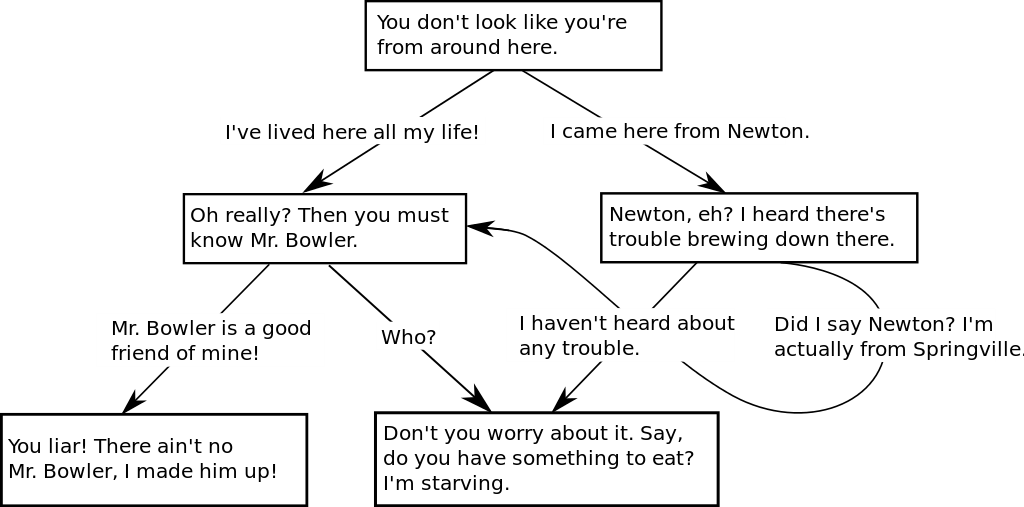
\includegraphics[width=0.38\textwidth]{SimpleStoryTree}
    \caption[]{Een simpele story graph. \footnotemark}
    \label{fig:simplestorytree}
\end{wrapfigure}
\footnotetext{Bron: \url{https://commons.wikimedia.org/wiki/File:Dialog_tree_example.svg}}


Veel interactieve verhalen met vertakkingen kunnen worden gerepresenteerd als een boom\cite{GalyeanIII1995}. Deze bestaat uit nodes (ook wel vertices genoemd) die de uitspraken/ terugkoppeling van de gesprekspartner representeren. Na de evaluatie van deze nodes kan er een keuze gemaakt worden. Deze discrete set van keuzes zijn terug te zien in de story tree als edges, hetgeen dat de nodes met elkaar verbindt. De gemaakte keuze bepaald de volgende node die geëvalueerd zal worden en dus de uitkomst van het verhaal. Dit formalisme laat ons toe om een inzichtelijk en simpele dialoog tussen twee personen te modelleren (\autoref{fig:simplestorytree}).

\subsubsection{Interactive behaviour trees}

% \begin{wrapfigure}{r}{0.4\textwidth}
%     \centering
%     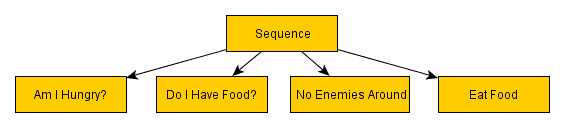
\includegraphics[width=0.38\textwidth]{BehaviourTreeSample}
%     \caption[]{Een voorbeeld van een behaviour tree. \footnotemark}
%     \label{fig:behaviourtreesample}
% \end{wrapfigure}
% \footnotetext{Bron: \url{https://www.gamasutra.com/blogs/ChrisSimpson/20140717/221339/Behavior_trees_for_AI_How_they_work.php}}

Interactive behaviour trees is een andere manier om een narratief te definiëren, welke gezien kan worden als een meer artificial intelligence (AI) georiënteerde oplossing. Hoewel story graphs direct en relatief simpel zijn is het hergebruik van nodes laag. Hierdoor resulteren uitgebreiden narrativen onderandere in onoverzichtelijke graphs. Het leren omgaan met interactive behaviour trees is relatief moeilijk, maar resulteert in een overzichtelijker en minder complexe structuur\cite{Kapadia2015}. 

\begin{figure}[htb]
    \centering
    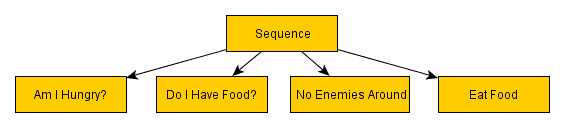
\includegraphics[width=0.45\textwidth]{BehaviourTreeSample}
    \caption[]{Een voorbeeld van een behaviour tree. \footnotemark}
    \label{fig:behaviourtreesample}
\end{figure}
\footnotetext{Bron: \url{https://www.gamasutra.com/blogs/ChrisSimpson/20140717/221339/Behavior_trees_for_AI_How_they_work.php}}

\subsection{Syntactische vormen}
\begin{wrapfigure}{r}{0.36\textwidth}
    \centering    
    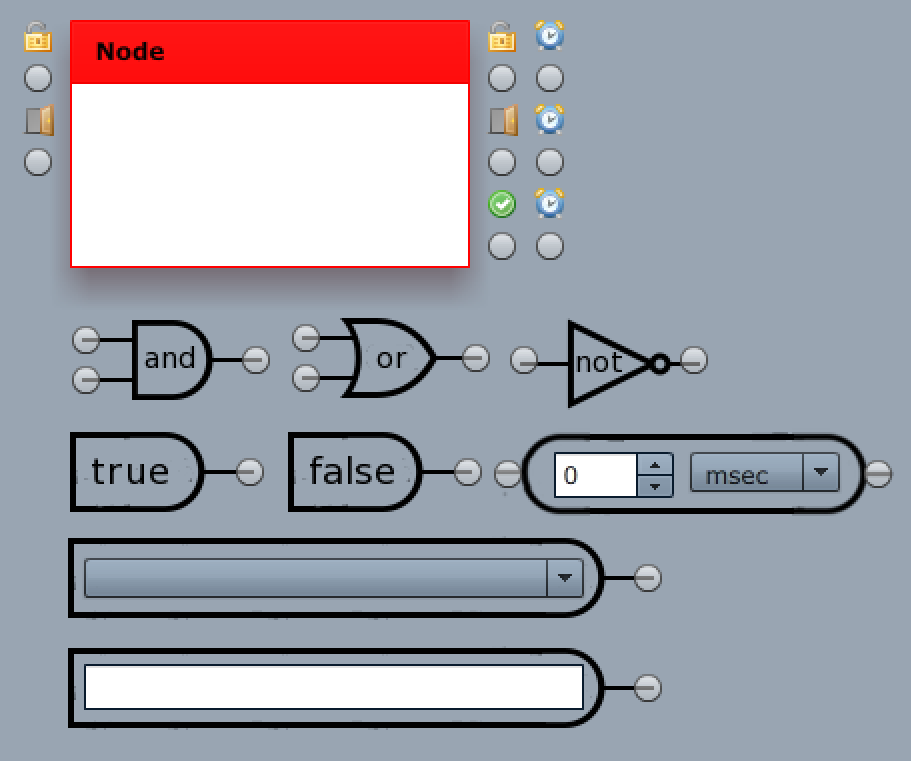
\includegraphics[width=0.32\textwidth]{SyntactischeVormen}
    \caption{Bouwblokken in de story editor.}
    \label{fig:syntactischevormen}
\end{wrapfigure}

Volgens formalisme kan een narratief uitgedrukt worden in syntactische vormen. Deze hebben verder geen waarde of betekenis, totdat er een interpretatie op losgelaten wordt. Een goed voorbeeld hiervan is terug te zien in de wiskunde. 

Zo bestaat de stelling van Pythagoras ook uit syntactische vormen die weergeven worden als letters:

\[ a^2 + b^2 = c^2 \]

Binnen de wiskunde hebben deze letters volgens het formalisme zelf geen betekenis. Dit wordt onderbouwd door het feit dat letters gebruikt kunnen worden voor andere stellingen, functies en vergelijkingen. De interpretatie op de eigenschappen van letter, zoals positie binnen de stelling, geven betekenis aan deze syntactische vorm.

Dit begrip komt ook terug in de editors in de vorm van nodes. Met deze nodes wordt er een narratief geformuleerd die de richtlijnen van het formalisme respecteert. We kunnen ook wel zeggen dat deze syntactische vormen bouwblokken zijn in de editors. In \autoref{fig:syntactischevormen} zijn enkele bouwblokken die in de story editor voorkomen te zien.

\section{Formalisme binnen de huidige editors}
De story- en dialog editor maken beide gebuikt van een ander formalisme. Dit is duidelijk te zien aan hoe het narratief representeert wordt door de editors (zie \autoref{fig:storyeditorvisualisationofstorydata} en \autoref{fig:dialogeditorvisualisationofstorydata}). 

\begin{figure}[H]
    \centering
    \begin{minipage}{.45\textwidth}
        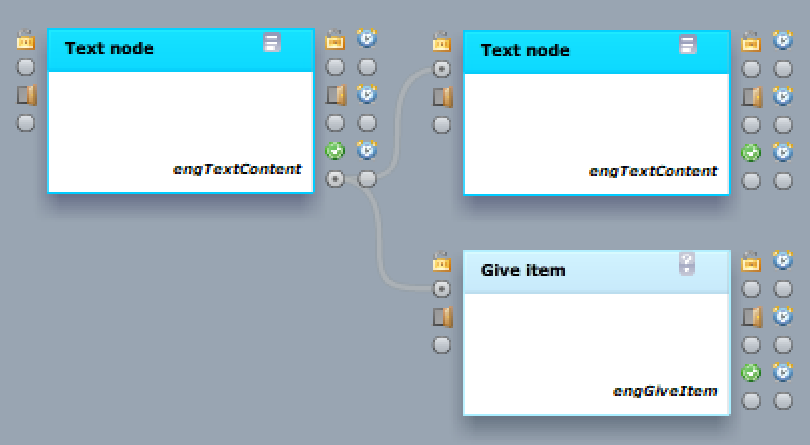
\includegraphics[height=0.45\linewidth]{StoryEditorVisualisationOfStoryData}
        \centering
        \caption{Story editor visualisatie\\ van achterliggende data.}
        \label{fig:storyeditorvisualisationofstorydata}
    \end{minipage}%
    \begin{minipage}{.45\textwidth}
        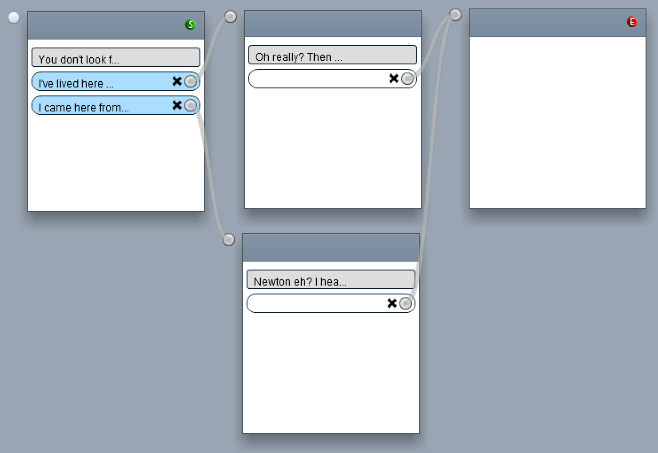
\includegraphics[height=0.45\linewidth]{DialogEditorVisualisationOfStoryData}
        \centering
        \caption{Dialog editor visualisatie\\ van achterliggende data.}
        \label{fig:dialogeditorvisualisationofstorydata}
    \end{minipage}
\end{figure}

Aan de huidige code base is te zien dat er een nauwe koppeling bestaat tussen de interface en het achterliggende formalisme. Dit maakt het lastig om meerdere formalismen te ondersteunen.

Dit kan een reden zijn geweest waarom er twee editors zijn opgezet; om de scheiding te maken tussen formalismen. Het is een uitdaging om in één omgeving meerdere formalismen te ondersteunen, omdat deze bestaat uit andere syntactische vormen en gebruik maken van andere principes.

Wel is het wenselijk om meerdere formalismen in één omgeving te ondersteunen om de volgende voorkomende problemen op te kunnen lossen:

\begin{itemize}
    \item Houdbaarheid; er hoeft nog maar één omgeving onderhouden te worden in plaats van twee wat scheelt in kosten.
    \item Houdbaarheid; generieke editor functionaliteit (copy/ paste, verplaatsen van nodes) kan worden hergebruikt en hoeft maar één keer geïmplementeerd te worden.
    \item Future proofing; benodigde formalismen kunnen in de toekomst worden toegevoegd. Er hoeft niet nog een nieuwe editor gemaakt te worden.
    \item Co-creatie; er zou eventueel een versimpeld formalisme toegevoegd kunnen worden waar klanten mee overweg kunnen. Hiernaast kan het versimpelde formalisme gebruikt worden om de volledige flow van het verhaal in kaart te brengen. Bij \&ranj is er al onderzoek gedaan naar formalisme voor klant co-creatie \cite{Schipper2015}.
\end{itemize}

\section{Formalisme scheiden van de editor}
Om een flexibele tool op te zetten voor het vertellen van diverse digitale interactieve verhalen is het nodig om verschillende formalisme voor diverse doeleinden te kunnen gebruiken. Met de toekomst blik van \&ranj en het ‘bad news’ dialoog moet er een formalisme ondersteund worden waarin een meer AI-benadering toegepast kan worden. Om dit mogelijk te maken moet er een manier komen om formalismen toe te kunnen voegen aan de editors.

Om de scheiding te leggen tussen de editor en het achter liggende formalisme zijn de volgende vragen opgesteld:

\begin{itemize}
    \item Hoe kunnen er bouwblokken worden geformuleerd per formalisme?
    \item Hoe kunnen er regels worden opgelegd aan het verbinden en het in elkaar voegen van deze bouwblokken?
    \item Hoe zou een algoritme eruitzien om vanuit een visuele structuur te compileren naar een formalisme?
\end{itemize}

\subsection{Het formuleren van bouwblokken}
\label{subsec:formulerenvanbouwblokken}
Ieder formalisme wordt ondersteund door syntactische vormen. Een concretere naam die aansluit bij de editors hiervoor is ‘bouwblokken’. Gebruikers van de editors zullen deze bouwblokken gebruiken om een narratief te definiëren volgens een vooraf vastgesteld formalisme. De representatie en interpretatie van deze bouwblokken verschillen dan ook per formalisme. Maar voor de editors zijn het allemaal ‘nodes’ (met eventuele porten) waarmee de node verbonden kan worden aan andere nodes; voor de editor hebben deze nodes geen verdere waarde noch betekenis. Als programmeur moet het mogelijk zijn om op een makkelijke manier bouwblokken te kunnen formuleren. Voor deze use case zijn de volgende requirements opgesteld:

\begin{enumerate}
    \item Ieder formalisme moet onderbouwd worden door een set aan bouwblokken, zodat de gebruiker deze kan gebruiken om binnen de richtlijnen van het formalisme te werken.
    \item Het constructie proces van de bouwblokken moet losstaan van de representatie, zodat verschillende representaties gebruikt kunnen worden voor diverse doeleinden.
    \item De representatie van deze bouwblokken moeten losgekoppeld worden van enige waarde of betekenis, zodat deze later volgens het formalisme geïnterpreteerd kunnen worden.
\end{enumerate}

\noindent De voornaamste manier om een node te construeren is om de bijbehorende klasse te instantiëren. Dit geeft ons een node object waarvan de representatie statisch is; het instantiëren van de node klassen resulteert altijd in hetzelfde object. Dit schendt requirements 2 en 3. Om constructie van representatie los te koppelen, en zo te voldoen aan de tweede requirement, kunnen er parameters in de constructor van de node klasse gedefinieerd worden die de eigenschappen en representatie van de node beschrijven. In \autoref{fig:storyeditorvisualisationofstorydata} is een van de bouwblokken in het formalisme van de story editor terug te zien: de ContentTypeNode. Dit bouwblok heeft een label en 8 porten. Het zojuist beschreven constructie proces voor deze node zou er als volgt uit kunnen zien:\\


\textbf{Functie handtekening}
\lstset{language=JavaScript,breaklines=true}
\begin{lstlisting}
    constructor Node(label: string, markup: string, allowBodyConnections: boolean, ports: Port[]): Node
\end{lstlisting}

\textbf{Voorbeeld}
\lstset{language=JavaScript,breaklines=true}
\begin{lstlisting}
    new Node('ContentType', '<rect class="node-body" width="100" height="100"><text/></rect>', false, [new Port(...), new Port(...), ...]);
\end{lstlisting}

\pagebreak
\noindent Deze manier van construeren heeft de volgende consequenties:
\begin{itemize}
    \item Een node moet geconstrueerd worden met argumenten die voldoen aan de parameters van de constructor. 
    \item Om achter de betekenis van de argumenten te komen moet er gekeken worden naar de constructor handtekening; argumenten zijn niet expliciet.
    \item Het stimuleert een nauwe koppeling tussen de node klasse en de achterliggende ‘diagramming library’ die de nodes visualiseert.
    \item Het stimuleert het aanroepen van het constructie proces op diverse plekken in de code.
    \item Er kunnen nodes worden gemaakt met verschillende representaties, door verschillende argumenten mee te geven.
\end{itemize}

\noindent Deze manier van construeren wordt al gauw ingewikkeld en onduidelijk ondervonden. Vooral omdat het constructie proces niet leesbaar en expliciet genoeg is. Daarnaast zal het constructie proces op verschillende plekken plaatsvinden, omdat er geen klasse bestaat die hier verantwoordelijk voor is. Dit heeft een grote invloed op de houdbaarheid van het product. Als er later een aanpassing aan een bouwblok gedaan moet worden zal dit relatief veel werk kosten en mogelijk fouten introduceren. Het constructie proces moet geabstraheerd worden, zodat het system onafhankelijk is van hoe de node objecten geïnstantieerd en gerepresenteerd worden. Door gebruikt te maken van ‘Creational design patterns’ kan er een abstractie laag worden geplaatst waardoor de gezochte scheiding kan worden gelegd\cite{DesignPatterns}.

Er is een kleine selectie aan patronen opgesteld die in aanmerking komen om het eerder beschreven probleem op te lossen. Deze design patterns zullen naast het probleem gelegd worden om de toepasselijkheid en consequenties in kaart te brengen. Uiteindelijk zal er een conclusie getrokken worden waarin het best passende design pattern ter sprake komt. De selectie aan design patterns die besproken zal worden bestaat uit:

\begin{itemize}
    \item Abstract factory
    \item Builder
    % \item Prototype
\end{itemize}

%% ABSTRACT FACTORY %%

\pagebreak
\subsubsection{Abstract factory}
\noindent\textbf{Intentie}\\
De intentie van dit patroon wordt beschreven als volgt\cite{DesignPatterns}\cite{SourceMakingAbstractFactory}:
\begin{quote} 
    \centering    
    \textit{
        "Provide an interface for creating families of related or depent objects without specifying their concrete classes."       
    }
\end{quote}

\noindent\textbf{Toepasselijkheid}\\
Dit patroon helpt de editor onafhankelijk zijn van de manier waarop de nodes geconstrueerd en gerepresenteerd worden \cite{DesignPatterns}, wat inhaakt op een deel van de tweede requirement. Verder is het wenselijk om meerdere formalismen te ondersteunen. Hierbij spelen bouwblokken een grote rol: deze ondersteunen het gebruik van een formalisme binnen de editor. Volgens de eerste requirement moet de editor een set aan bouwblokken kunnen aanbieden die de gebruiker kan gebruiken. Het abstract factory patroon maakt het mogelijk om families van nodes te creëren \cite{DesignPatterns}. Hierbij is de familie het formalisme.
\newline

\noindent\textbf{Structuur}

\begin{figure}[H]
    \centering    
    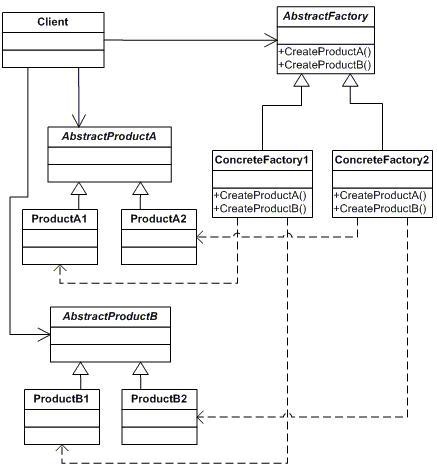
\includegraphics[width=0.55\textwidth]{AbstractFactoryUML}
    \caption[]{Klasse diagram van het abstract factory pattern. \footnotemark}
    \label{fig:abstractfactoryuml}
\end{figure}
\footnotetext{Bron: \url{http://www.dofactory.com/net/abstract-factory-design-pattern}}

\pagebreak
\noindent\textbf{Deelnemers}
\begin{itemize}
    \item \textbf{AbstractFactory} (NodeFactory)
    \begin{itemize}
        \item Biedt een interface aan met methodes voor het maken van node objecten.
    \end{itemize}

    \item \textbf{ConcreteFactory} (StateMachineNodeFactory, BehaviourTreeNodeFactory)
    \begin{itemize}
        \item Implementeert de ‘NodeFactory’ om concrete node objecten te kunnen maken.
    \end{itemize}

    \item \textbf{AbstractProduct} (Node, mogelijke extra abstractie laag: StateMachineNode, BTNode ...)
    \begin{itemize}
        \item Biedt de interface voor een type van concrete node objecten.
    \end{itemize}
    \item \textbf{ConcreteProduct} (ContentNode, SelectorNode, ...)
    \begin{itemize}
        \item Implementeert ‘Node’ en maakt onderscheid tussen verschillende type nodes mogelijk.
        \item Definieert een product dat gemaakt zal worden door het desbetreffende concrete factory object.
    \end{itemize}
    \item \textbf{Client}
    \begin{itemize}
        \item Gebruikt de interfaces die gedefinieerd zijn door de ‘AbstractFactory’ en de ‘AbstractProduct’ klassen.
    \end{itemize}
\end{itemize}

\noindent\textbf{Consequenties}
\begin{itemize}
    \item Het isoleert de concrete node klassen; de factory heeft de verantwoordelijkheid en het proces om nieuwe nodes te maken.
    \item Het maakt het verwisselen van verschillende formalisme makkelijk; Elk formalisme zou een eigen factory kunnen hebben. De factory wordt op één plek in de code geïnstantieerd en omdat de concrete factories allemaal dezelfde interface implementeren kunnen we makkelijk van concrete factory verwisselen.
    \item Het dwingt het implementeren van interface af; elke concrete node zal de node interface moeten implementeren. Om subklasse specifieke operaties aan te kunnen roepen zal er gebruik gemaakt moeten worden van casting.
    \item Nieuwe nodes toevoegen is lastig; per type node zal er een methode bijkomen in zowel de abstract factory als de concrete factories. Hiernaast kan dit zorgen voor concrete factories die operaties bevatten met een lege body, omdat bepaalde type nodes niet van toepassing zijn in het formalisme dat de concrete factory ondersteund.
\end{itemize}

\noindent\textbf{Abstract Factory conclusie}\\
Het is wenselijk om het constructie proces te isoleren en te scheiden van de rest van de applicatie. Dit maakt het makkelijker om later eventueel van diagramming library te wisselen en nodes aan te passen. Verschillende implementaties van ‘AbstractFactory’ kunnen ieder nodes voor een formalisme aanbieden. Echter omdat elke ‘ConcreteFactory’ de ‘AbstractFactory’ implementeert zullen deze moeten voldoen aan de interface van de geabstraheerde factory. Dit kan zorgen voor lege methodes die verder geen waarde hebben. Hiernaast kan dit de illusie wekken dat elke node terugkomt in ieder formalisme. Tenslotte is het toevoegen van nieuwe nodes lastig. Volgens de eerste requirement moet er een set aan bouwblokken aangeboden worden. Als er nieuwe bouwblokken in de vorm van nodes aan de set toegevoegd moeten worden zal de interface van de ‘AbstractFactory’ ook aangepast moeten worden. Dit heeft als gevolg dat iedere ‘ConcreteFactory’ deze nieuwe methode ook moet implementeren. Hoe meer formalismen er zijn, des te moeilijker het zal zijn om nieuwe bouwblokken toe te voegen. Dit maakt het ‘Abstract Factory’ design pattern ongeschikt voor deze use case.

\pagebreak
%% BUILDER %%
\subsubsection{Builder}
\noindent\textbf{Intentie}\\
De intentie van dit patroon wordt beschreven als volgt\cite{DesignPatterns}\cite{SourceMakingBuilder}:
\begin{quote} 
    \centering    
    \textit{
        "Separate the construction of a complex object from its representation so that the same construction process can create different representations."        
    }
\end{quote}

\noindent\textbf{Toepasselijkheid}\\
Het builder patroon is interessant omdat nodes een vrij complex object zijn die meerdere representaties zal hebben in de editor. Er moeten verschillende bouwblokken ondersteund worden (requirement 1) die ieder een eigen presentatie hebben (requirement 2). Hiernaast maakt het patroon het constructie proces expliciet door een interface aan te bieden waarmee nodes opgebouwd kunnen worden.
\newline

\noindent\textbf{Structuur}

\begin{figure}[H]
    \centering    
    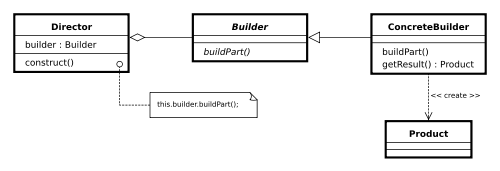
\includegraphics[width=0.7\textwidth]{BuilderUML}
    \caption[]{Klasse diagram van het builder pattern. \footnotemark}
    \label{fig:builderyuml}
\end{figure}
\footnotetext{Bron: \url{https://en.wikipedia.org/wiki/Builder_pattern}}

\noindent\textbf{Deelnemers}
\begin{itemize}
    \item \textbf{Builder} (NodeBuilder)
    \begin{itemize}
        \item Biedt een interface voor het maken van node onderdelen (e.g. porten, labels, visuals).
    \end{itemize}

    \item \textbf{ConcreteBuilder} (StateMachineNodeBuilder, BehaviourTreeNodeBuilder)
    \begin{itemize}
        \item Implementeert de ‘Builder’ interface en maakt het mogelijk om onderdelen te maken.
        \item Definieert en houdt bij hoe de representatie gemaakt wordt. 
        \item Biedt een interface om de uiteindelijke node te verkrijgen.

    \end{itemize}

    \item \textbf{Director} (StateMachineDirector, BehaviourTreeDirector)
    \begin{itemize}
        \item Gebruikt de ‘Builder’ interface om de verschillende bouwblokken per formalisme te construeren.
    \end{itemize}
    \item \textbf{Product} (ContentNode, SelectorNode, ...)
    \begin{itemize}
        \item Representeert de node waaraan de ‘ConcreteBuilder’ bouwt.
        \item Bevat de aangebouwde onderdelen en achterliggende model (e.g. content type of een expressie).
    \end{itemize}
\end{itemize}

\pagebreak
\noindent\textbf{Consequenties}
\begin{itemize}
    \item Het isoleert het constructie proces en de representatie van nodes; de node editor hoeft niet te weten hoe een node gemaakt en gerepresenteerd wordt. De builder biedt een interface voor het construeren van nodes die de concrete builder implementeert. Deze code om nodes te creëren hoeft maar één keer geschreven te worden. Directors kunnen deze interface gebruiken om verschillende varianten van nodes te maken.
    \item Het constructie proces van nodes is explicieter; de builder biedt een interface met methodes die direct beschrijven welk onderdeel er gemaakt wordt. Zo is de constructie die plaats vindt in \autoref{lst:builderconstruction} explicieter dan \autoref{lst:constructionbyconstructor}.
    \item Fijnere controle over constructie proces van nodes; nodes worden stap voor stap in elkaar gezet. In tegenstelling tot andere creational design patterns worden nodes niet in één keer gemaakt.
\end{itemize}

\lstset{language=JavaScript}
\begin{lstlisting}[caption={Constructie stap voor stap door de 'Director', geschreven in TypeScript.},captionpos=b,label={lst:builderconstruction}]
    return this._builder
        .build<ContentNode>()
        .label('ContentNode')
        .addPort(UnlockPort)
        .addPort(CompletedPort)
        .getNode();
\end{lstlisting}

\lstset{language=JavaScript}
\begin{lstlisting}[caption={Directe instantiatie door constructor.},captionpos=b,label={lst:constructionbyconstructor}]
    return new Node('ContentNode', [new Port(...)]);
\end{lstlisting}

\noindent\textbf{Builder conclusie}\\
\begin{wrapfigure}{r}{0.4\textwidth}
    \centering    
    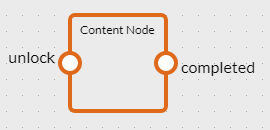
\includegraphics[width=0.38\textwidth]{PrototypeSimpleContentNode}
    \caption{Prototype resultaat van \autoref{lst:builderconstruction}}
\end{wrapfigure}
Het builder patroon biedt de mogelijkheid om nodes stapsgewijs te construeren. Door middel van de interface die de ‘NodeBuilder’ klasse biedt kunnen nodes expliciet en modulair opgebouwd worden (zie \autoref{lst:builderconstruction}). Dit maakt het makkelijk om nieuwe bouwblokken te definiëren, zonder iets af te weten van hoe de nodes gemaakt worden. Deze code is één keer geschreven en bevind zich in de concrete builders. De ‘Director’ klasse kan geabstraheerd worden die per formalisme geïmplementeerd kan worden. Deze concrete directors kunnen een set aan bouwblokken opbouwen die makkelijk aan te passen is, waarmee voldaan wordt aan de eerste requirement. Het patroon biedt ook een fijnere controle over het constructie proces, omdat nodes stapsgewijs op gebouwd kunnen worden. Dit maakt het makkelijk om bouwblokken met verschillende representaties te creëren en hiermee wordt voldaan aan de tweede requirement.

\pagebreak
\subsection{Het opleggen van restricties}

% \begin{wrapfigure}{r}{0.2\textwidth}
%     \centering    
%     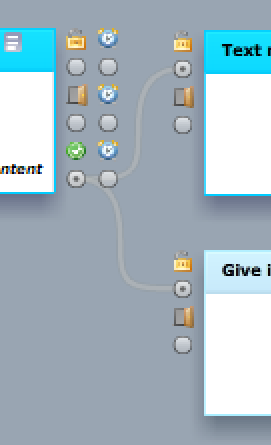
\includegraphics[width=0.18\textwidth]{StoryEditor_LinksBetweenNodes}
%     \caption{Verbonden porten in de huidige story editor.}
%     \label{fig:linksinstoryeditor}
% \end{wrapfigure}

Door de bouwblokken aan elkaar te kunnen verbinden kunnen er een of meerdere verhaallijnen worden gemoduleerd. Verschillende bouwblokken worden met elkaar verbonden om volgorde en relatie tussen elkaar aan te geven. 

Formalismen leggen restricties op zowel het verbinden als het in elkaar voegen van bouwblokken. Dit kan duidelijk teruggezien worden in de huidige editors. Hierin wordt er gebruik gemaakt van porten om de nodes met elkaar te verbinden (\autoref{fig:linksinstoryeditor}). Zowel de story- als dialog editor lijkt gebruik te maken van semantische port groepen. Dit maakt het mogelijk om een betekenis te geven aan de porten. Beide hebben een 'in' en 'uit' groepen, waarbij de er geen verbinden kunnen worden gevormd tussen dezelfde groep; 'in' kan niet verbonden worden met een andere 'in'. Hiernaast werken sommige porten met tijd (zie de porten met klokjes in \autoref{fig:linksinstoryeditor}) en andere met logische expressies.

% \begin{wrapfigure}{r}{0.32\textwidth}
%     \centering    
%     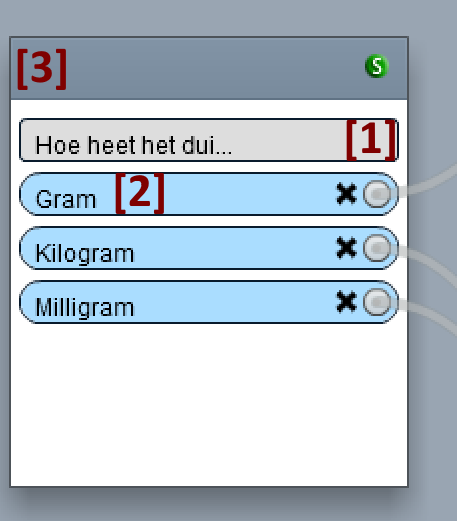
\includegraphics[width=0.28\textwidth]{DialogStateNodeEmbedding}
%     \caption{Dialog editor: bouwblokken gevoegd in andere bouwblokken.}
%     \label{fig:embeddedcomponents}
% \end{wrapfigure}

In de dialog editor kunnen bouwblokken in elkaar gevoegd worden (zie \autoref{fig:embeddedcomponents}). Hier zitten wel bepaalde regels aan vast. Zo kunnen er alleen 'commands' (1) en 'options' (2) gevoegd worden in een 'state' (3). De 'command' en 'option' bouwblokken kunnen alleen bestaan als ze gevoegd zijn.

\begin{figure}[H]
    \centering
    \begin{minipage}{.45\textwidth}
        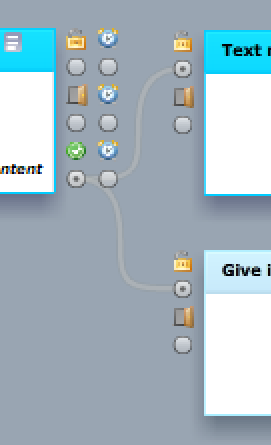
\includegraphics[height=0.65\linewidth]{StoryEditor_LinksBetweenNodes}
        \centering
        \caption{Verbonden porten in\\ de huidige story editor.}
        \label{fig:linksinstoryeditor}
    \end{minipage}%
    \begin{minipage}{.45\textwidth}
        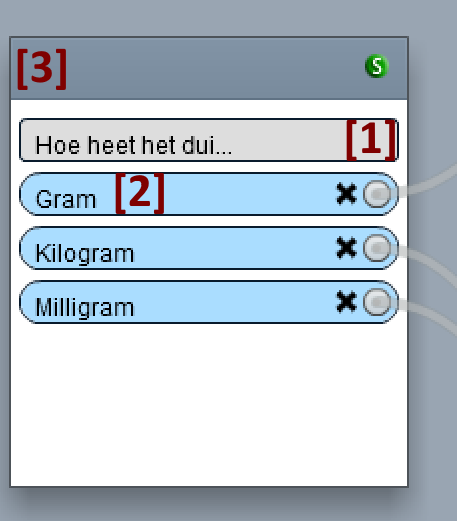
\includegraphics[height=0.65\linewidth]{DialogStateNodeEmbedding}
        \centering
        \caption{Dialog editor: bouwblokken gevoegd\\ in andere bouwblokken.}
        \label{fig:embeddedcomponents}
    \end{minipage}
\end{figure}

\clearpage
\subsubsection{Het valideren van verbindingen}
\noindent\textbf{Niveau}\\
Eerst moet er gekeken worden naar op welke niveau gevalideerd moet worden. Het niveau bepaald de granulariteit waarop de controle uitgevoerd wordt. Als er gekeken wordt op groepsniveau is het makkelijker om de rule set, of terwijl de verschillende restrictie regels, overzichtelijk en houdbaar in te delen. Hiertegenover staat dat er sprake is van een validatie op hoog niveau. Er wordt gekeken naar semantische groepen en niet naar de individuele porten. Dit maakt het moeilijk om eventuele uitzonderingen in de restricties toe te laten. Veel uitzonderingen kunnen echter weer zorgen voor onoverzichtelijkheid.

Het vastleggen van een rule set op groep niveau bevorderd de houdbaarheid, maar maakt het systeem ook minder flexibel. Het uitgangspunt van dit onderzoek is om alles zo flexibel mogelijk op te zetten, zolang dit geen hevige negatieven gevolgen heeft. Daarom zal het werken met semantische port groepen worden gestimuleerd, maar wanneer er een fijnere maten van controle vereist is moet het mogelijk zijn om op individueel niveau te valideren. Hierbij zal de validatie op individueel niveau de groepsvalidatie overschrijven.
\newline

\noindent\textbf{Validatie}\\
Om volledige controle te geven over het validatie proces zal het systeem gebruik maken van een validatie functie. Deze functie zal worden uitgevoerd wanneer de gebruiker een verbindingen gaat maken. De validatie functie kan uitgedrukt worden als:

\begin{quote} 
    \centering    
    \textit{
        validate: (x) =\textgreater{} boolean
    }
\end{quote}

\begin{wrapfigure}{r}{0.4\textwidth}
    \centering    
    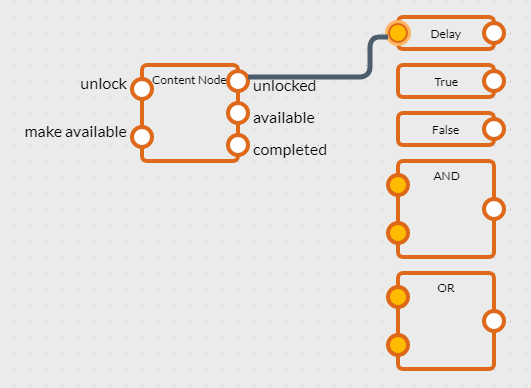
\includegraphics[width=0.38\textwidth]{PrototypeValidation}
    \caption{Validatie in het prototype; mogelijke porten worden gemarkeerd}
    \label{fig:prototypevalidation}
\end{wrapfigure}

Hierbij is 'x' het gene waar de verbinding tegen gevalideerd wordt. Omdat formalismen directe verbindingen met andere porten zouden kunnen toelaten, en het systeem hier geen restricties op moet leggen, kan 'x' zowel een port als een node zijn. Dit introduceert een nieuw probleem, omdat we niet weten wat voor type object meegegeven wordt als argument. Het maken van een validatie functie is lastig als het niet duidelijk is waartegen gevalideerd gaat worden. Echter is dit in een statically typed language, een programmeertaal waarin variabelen bestaan uit een type en een waarde, op te lossen door middel van method overloading. Hierbij wordt er voor elke mogelijke input een methode gemaakt (in dit geval twee methodes). Tijdens het compileren wordt er beslist welke methode waar gebruikt wordt. In een dynamically typed language bestaat het concept method overloading niet, omdat variabelen niet gebonden zijn aan een type. Dit betekent dat Typescript, wat uiteindelijk omgezet wordt in Javascript (een dynamically typed language), geen gebruik kan maken van method overloading. Echter biedt Javascript een uitweg met de 'instanceof' operator. Deze operator geeft een boolean, een logische waarde, terug die waar zal zijn als de constructor van het type terugkomt in de prototype chain. Een voorbeeld van een validatie functie geschreven in Typescript is terug te zien in 
\autoref{lst:validationfunction}. Deze functie beschrijft dat er alleen een verbinding mag worden gelegd met andere Nodes. Als er een validatie functie gedefinieerd is op individueel niveau zal deze de groepsvalidatie functie overschrijven. Als de uitkomst van deze functie 'true' is wordt de port gemarkeerd (\autoref{fig:prototypevalidation}).

\pagebreak
\lstset{language=JavaScript}
\begin{lstlisting}[caption={Een voorbeeld van een validatie functie in Typescript.},captionpos=b,label={lst:validationfunction}]
    validateConnection(against: Port | Node): boolean => {
        if (against instanceof Port) {
            return false;
        }

        if (against instanceof Node) {
            return true;
        }
    }
\end{lstlisting}

\subsubsection{Het valideren van het in elkaar voegen}
Dezelfde methode en techniek kan gebruikt worden ter validatie van het in elkaar voegen van nodes. Hierbij is ‘against’ parameter altijd een andere node.

\pagebreak
\subsection{Het compileren van een visuele structuur}
\label{subsec:hetcompilerenvaneenvisuelestructuur}
Nadat het verhaal geschreven is in de editor wordt deze geëxporteerd zodat het NGT hiervan gebruik kan maken. Dit exporteer proces zet de visuele structuur om naar JavaScript Object Notation (JSON), een gestandaardiseerd dataformaat. Het NGT kan dit formaat uitlezen en interpreteren. Tijdens dit compilatie proces wordt editor specifieke informatie, zoals de positie en uiterlijk van nodes, niet mee geëxporteerd. Voor het NGT heeft deze informatie geen waarde en is dus overbodig.

\subsubsection{Het scheiden van bouwblokken en waarde}
In de huidige editors zit het formalisme vast gebakken in de visuele structuur. Bouwblokken hebben naast een uiterlijk ook een methode die een JavaScript object met data vrijgeeft. Dit object wordt vervolgens direct geserialiseerd; omgezet naar een formaat dat opgeslagen kan worden. De editor koppelt dus waarde en formalisme aan de bouwblokken zelf. Dit resulteert in niet herbruikbare bouwblokken; de bouwblokken zijn direct gekoppeld aan het formalisme.

Om het hergebruik van bouwblokken tussen meerdere formalismen mogelijk te maken moet de waarde van de bouwblokken gescheiden worden. Bouwblokken kunnen theoretisch terugkomen in meerdere formalismen waarin ze anders geïnterpreteerd moeten worden. Zo kunnen content typen terugkomen in zowel het formalisme van de story- als dialog editor. In de story editor zijn content typen terug te zien in de vorm van nodes, met verschillende in en uit porten (\autoref{fig:storyeditorcontenttype}). De dialog editor gebruikt content typen zonder porten (\autoref{fig:dialogeditorcontenttype}). Hier zijn de content typen ingevoegd in andere nodes.

\begin{figure}[H]
    \centering
    \begin{minipage}{.45\textwidth}
        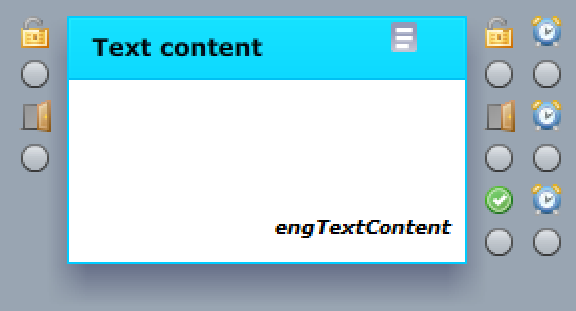
\includegraphics[height=0.45\linewidth]{StoryEditor_Node}
        \centering
        \caption{Een content type in\\ de story editor.}
        \label{fig:storyeditorcontenttype}
    \end{minipage}%
    \begin{minipage}{.45\textwidth}
        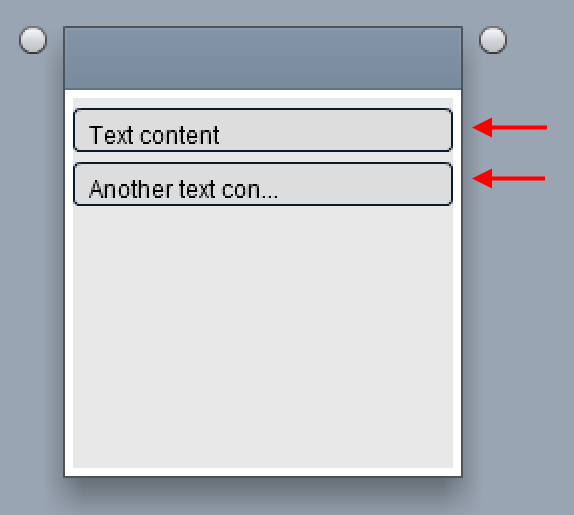
\includegraphics[height=0.55\linewidth]{DialogEditor_Node}
        \centering
        \caption{Een content type in\\ de dialog editor.}
        \label{fig:dialogeditorcontenttype}
    \end{minipage}
\end{figure}

% \begin{figure}[htb]
%     \centering    
%     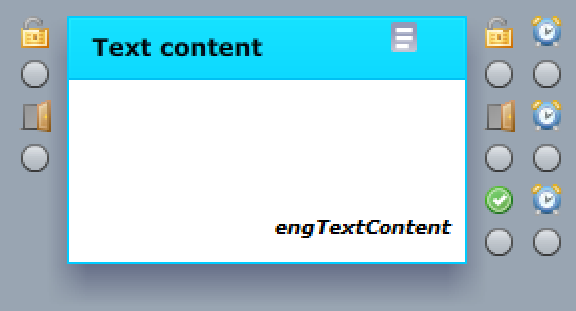
\includegraphics[width=0.45\textwidth]{StoryEditor_Node}
%     \caption{Een content type in de story editor.}
%     \label{fig:storyeditorcontenttype}
% \end{figure}

% \begin{figure}[htb]
%     \centering    
%     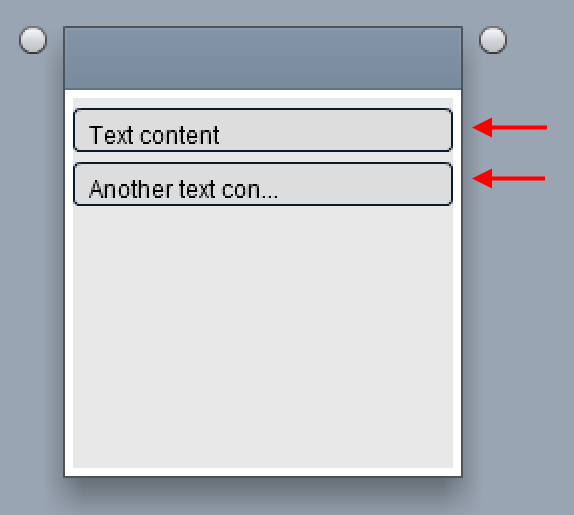
\includegraphics[width=0.45\textwidth]{DialogEditor_Node}
%     \caption{Een content type in de dialog editor.}
%     \label{fig:dialogeditorcontenttype}
% \end{figure}

\noindent In \autoref{subsec:formulerenvanbouwblokken} wordt representatie van bouwblokken losgekoppeld van de werking door gebruik te maken van het ‘builder’ design pattern. De volgende stap is om de visuele structuur om te zetten naar een export-bestand volgens de richtlijnen van het desbetreffende formalisme. Hiervoor moet de serialisatie logica losgetrokken worden van de nodes zelf, zodat nodes geïnterpreteerd kunnen worden volgens het formalisme. Wanneer het verhaal wordt gecompileerd moet er volgens de richtlijnen van het formalisme waarde gekoppeld worden aan de bouwblokken. Hiernaast moet er worden gekeken hoe de graaf doorlopen gaat worden.

\pagebreak
\subsubsection{Compilatie stap}
De interpretatie van nodes moet losgekoppeld worden van de visuele structuur. Dit betekent dat de nodes zelf geen methode moeten bevatten die de data van een node vrijgeeft. Nodes moeten geïnterpreteerd worden volgens zowel interface als formalisme. 

Door gebruikt te maken van het visitor design pattern wordt er een context aangeboden waarin het exporteer-bestand opgebouwd kan worden. De 'gang of four' koppelt de volgende intent aan dit design pattern\cite{DesignPatterns}:

\begin{quote} 
    \centering    
    \textit{
        "Represent an operation to be performed on the elements of an object structure. Visitor lets you define a new operation without chaning the classes of the elements on which it operates."     
    }
\end{quote}

Deze intentie kan gekoppeld worden aan het eerder beschreven probleem. De operatie die uitgevoerd wordt op de elementen van een object structuur, betreft het omzetten van de visuele structuur naar een export-bestand. Hierbij worden operaties gedefinieerd in de visitor in plaats van in de nodes zelf waarmee interpretatie van de nodes losgekoppeld wordt.

\subsubsection{Visitor pattern}
Het visitor pattern definieert de volgende deelnemers:

\begin{itemize}
    \item \textbf{Visitor} (ExportGeneratingVisitor)
    \begin{itemize}
        \item Definieert voor iedere concrete element klasse in de datastructuur een 'Visit' methode. Echter werken we met JavaScript, een programmeertaal die loosly typed is; data typen worden niet expliciet gedefinieerd. Hierdoor kan er geen gebruik worden gemaakt van method overloading. Dit heeft als gevolg dat de Visitor interface maar één 'Visit' methode zal definieren. In de concrete visitor zullen de type specifieke operaties worden gedefinieerd.
    \end{itemize}

    \item \textbf{Concrete Visitor} (StoryExportGeneratingVisitor)
    \begin{itemize}
        \item Implementeerd de 'Visitor' interface en biedt content voor het algoritme. Hiernaast kan de concrete visitor staat verzamelen, in dit geval bouwt deze het export-bestand op.
    \end{itemize}

    \item \textbf{Element} (Node)
    \begin{itemize}
        \item Definieert een 'Accept' methode met de Visitor als parameter.
    \end{itemize}

    \item \textbf{ConcreteElement} (Bouwblokken in formalisme, zoals 'ContentNode')
    \begin{itemize}
        \item Implementeert de 'Element' interface, met de 'Accept' methode die een visitor as parameter neemt.
    \end{itemize}

    \item \textbf{ObjectStructure} (Graph)
    \begin{itemize}
        \item Biedt een interface om te itereren over haar elementen.
    \end{itemize}
\end{itemize}

\noindent Het totaal plaatje is terug te zien in \autoref{fig:appliedvisitorpaternuml}. Voor ieder formalisme wordt een concrete visitor aangemaakt, zodat ieder formalisme de elementen kan interpreteren volgens haar eigen richtlijnen.

\begin{figure}[htb]
    \centering    
    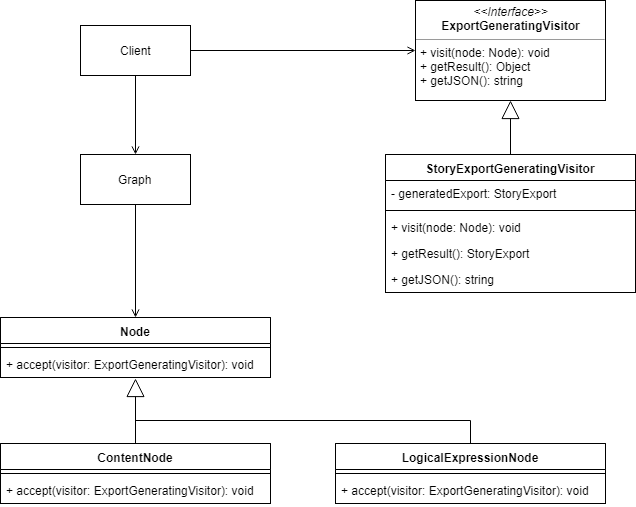
\includegraphics[width=0.9\textwidth]{ExportGeneratingVisitor}
    \caption{Het visitor pattern toegepast voor het formalisme van de story editor.}
    \label{fig:appliedvisitorpaternuml}
\end{figure}

\pagebreak
\subsubsection{Consequenties}
Het gebruik van het visitor pattern om van visuele structuur naar export-bestand te compileren heeft de volgende consequenties:
\begin{enumerate}
    \item Bouwblokken kunnen worden toegevoegd aan een formalisme, zonder zelf van het formalisme af te weten. Hiermee wordt vervuiling van de nodes voorkomen. 
    \item Bouwblokken kunnen worden hergebruikt in andere formalisme. De concrete visitor voor het desbetreffende formalisme moet dan wel een methode definiëren die de bouwblokken kan bezoeken.
    \item Elke bouwblok moet een ‘Accept’ methode implementeren.
    \item Concrete visitors kunnen staat bijhouden. Dit wordt gebruikt om het export-bestand op te bouwen.
\end{enumerate}

\noindent In een strongly typed programmeertaal zou het toevoegen van concrete elementen lastiger zijn. Hiervoor moet de interface van de visitor aangepast worden om het nieuwe element te ondersteunen. Dit zou ook betekenen dat iedere concrete visitor (en dus elk formalisme) een visit methode zou moeten implementeren voor ieder bouwblok. Als bouwblokken niet worden gebruikt in een formalisme zou dit lege methode opleveren. Echter wordt deze consequentie ontweken doordat er gewerkt wordt in JavaScript, een loosly typed programmeertaal.

Het prototype implementeert het visitor pattern en valideert zo het gebruik van het visitor pattern voor de compilatie stap.

\pagebreak
\section{Conclusie}
Met dit hoofdstuk wordt de volgende deelvraag beantwoord: “Hoe kan de architectuur achter de editor zo worden opgezet dat er in latere stadia nieuwe narratieve formalismen makkelijk doorgevoerd kunnen worden?”.

Een formalisme bestaat (1) uit syntactische vormen en legt (2) restricties op het verbinden en het in elkaar voegen van deze vormen. Met behulp van het builder design pattern kunnen bouwblokken worden gescheiden van representatie. Dit laat het hergebruik van bouwblokken met verschillende representaties toe. Hiernaast biedt de builder een expliciete interface voor het construeren van nodes en kapselt deze het constructieproces af. Ieder formalisme beschikt over een eigen director die een set aan beschikbare bouwblokken formuleert voor het desbetreffende formalisme.

Restricties tussen het verbinden van deze syntactische vormen kunnen worden opgelegd door gebruik te maken van een validatie functie. Wanneer de bouwblokken gebruik maken van porten worden er semantische port groepen gedefinieerd om restricties op groepsniveau toe te laten. Restricties op individueel niveau overschrijven de restricties gedefinieerd op groepsniveau. 

De visuele weergave van bouwblokken kan worden losgekoppeld van één ingebakken formalisme door gebruik te maken van het visitor design pattern. Hierdoor worden bouwblokken en waarde losgekoppeld. Tijdens het compileren van de visuele structuur naar een export-bestand zal er waarde worden gehangen aan de bouwblokken volgens de richtlijnen van het desbetreffende formalisme. Dit laat het hergebruiken van bouwblokken tussen verschillende formalismen toe.

Door formalisme specifieke logica los te koppelen van de visuele weergave van bouwblokken kunnen er in latere stadia nieuwe bouwblokken geformuleerd worden en nieuwe formalisme doorgevoerd worden.